\documentclass{desyproc}

\def\al{\alpha}
\def\ga{\gamma}
\def\rh{\varrho}
\def\th{\vartheta}
\def\be{\beta}
\def\ph{\varphi}
\def\De{\Delta}
\def\Ph{\Phi}
\def\si{\sigma}
\def\un#1{\ {\rm #1}}
\def\subtitle#1#2{\vbox{\setbox0\hbox{#1}\copy0\hbox to\wd0{\hss#2\hss}}}
\def\d{{\rm d}}
%\def\log{\mathop{\rm log}}

\begin{document}
%------------------------------------
\title{TOTEM Experiment: Elastic and Total Cross Sections}

\author{{\slshape J. Ka\v spar on behalf of the TOTEM Collaboration}\\[1ex]
CERN, Geneva and Institute of Physics of the AS CR, Prague}

% if the proceedings are available online (e.g. at Indico)
% please enter the contribution ID or file_name below for the DOI
%\contribID{32}
\contribID{JanKaspar\_EDS09}

% TO THE CONFERENCE EDITORS: 
% please update the following information      
% before sending the template to the authors
% \confID{800}  % if the conference is on Indico uncomment this line
\desyproc{DESY-PROC-2009-xx}
\acronym{EDS'09} % if you want the Acronym in the page footer uncomment this line
\doi  % if there is an online version we will register DOIs

\maketitle

\begin{abstract}
The physics programme and the detector apparatus of the TOTEM experiment is presented. Then, the key optics and their goals are summarized. The method to measure the total pp cross section is introduced. One of its essential parts, the extrapolation to $t=0$, is discussed in detail and extrapolation strategies for $\be^*=1535$ and $90\un{m}$ optics are presented. In particular, an adequate parameterization and a treatment of Coulomb scattering is proposed. In the last section, a Roman Pot alignment procedure is described.
\end{abstract}

\vskip-9pt\vskip0pt
\section{Introduction}\label{sec:intro}

The TOTEM experiment \cite{tdr,jinst} is dedicated to forward hadronic phenomena. The tree pillars of its physics programme are: an accurate measurement of the total $\rm pp$ cross section, a measurement of elastic scattering in a wide kinematic range and studies of diffractive processes. This paper is focused on the first two, for the latter one we refer to \cite{tdr, jinst, simone}.

The programme is touching one of the least explored and understood areas of hadronic physics. This fact can be well demonstrated by Fig.~\ref{fig:why}. The left plot shows several model predictions for elastic differential cross sections which differ by several orders of magnitude at large $|t|$ (four-momentum transfer squared). The right figure compiles data on the total pp cross section. Due to large uncertainties of cosmic ray experiments and conflicting Tevatron data \cite{tevatron1,tevatron2}, this data set can hardly favor any of the proposed theoretical descriptions over another. TOTEM shall shed some light onto those open questions by providing precise measurements -- see for instance the anticipated error bar for total cross section in Fig.~\ref{fig:why}.

\begin{figure}[htb]
\centerline{\hss
	\includegraphics[height=0.4\textwidth]{../fig/elasticCrossSection_withAcceptance_bw}\hfil
	\includegraphics[height=0.4\textwidth]{../fig/sigma_tot}\hss
}%
\vskip-3mm
\caption{Left: predictions of the elastic differential cross-section at a center-of-mass energy of $14\un{TeV}$ by several phenomenological models. Acceptance bands for the main optics (see Sec.~\ref{sec:meas}) are shown at the bottom. Right: a compilation of available data for the total pp cross section with a fit by the COMPETE collaboration \cite{cudell}. The anticipated ultimate precision ($1\%$) is shown in the bottom right corner.}%
\label{fig:why}%
\end{figure}

The challenging programme brings special requirements for the detector apparatus. In particular, {\em large pseudorapidity coverage} -- to detect most fragments from inelastic collisions and excellent {\em acceptance for outgoing diffractive and elastic protons}. To accomplish this task, TOTEM comprises three subdetectors: the inelastic telescopes T1 and T2 and a system of Roman Pots (RP) for proton detection. For details on instrumentation see \cite{tdr, jinst, gennaro}. This design results in a unique apparatus with an excellent pseudorapidity coverage, see Fig.~\ref{fig:acceptance}. The acceptance of the RPs can be further varied by using different optics, as will be discussed in the next section.

\begin{figure}[htb]
\centerline{\hss
	\includegraphics[height=0.4\textwidth]{../fig/acceptanceOverview_bw}\hfil
	\includegraphics[height=0.4\textwidth]{../fig/elasticAcceptance_bw}\hss
}%
\vskip-3mm
\caption{The acceptance of the TOTEM apparatus. Left: The coverage of the three subsystems of TOTEM. The shown acceptance of RPs refers to the $\be^*=1535\un{m}$ optics. For the other optics, the acceptance is shifted to lower pseudorapidity values, which narrows the gap between RPs and T2. Right: RP acceptances for elastic events for different optics at $\sqrt{s}=14\un{TeV}$.}%
\label{fig:acceptance}%
\end{figure}




%%%%%%%%%%%%%%%%%%
\section{Measurement of the total cross section}
\label{sec:meas}

The forward protons will be detected by the system of Roman Pots. Their position and acceptance depends on the settings of the accelerator (beam optics) -- for details see chapter~6 in \cite{jinst}. TOTEM plans to exploit the following 3 types of optics.
%(they can be categorized by corresponding value of $\be^*$)

\begin{enumerate}
\item {\em $\be^* = 1535\un{m}$}. This is the ultimate optics for low $|t|$ elastic scattering and precise ($1\%$ error) total cross section measurement.
\item {\em $\be^* = 90\un{m}$} is a universal optics allowing for measurement of elastic scattering (medium $|t|$ range), total cross section ($5\%$ uncertainty) and also for diffraction studies.
\item {\em $\be^* = 0.5 \div 3\un{m}$} (standard optics) are suited for high $|t|$ elastic scattering and various diffractive measurements.
\end{enumerate}

See Figs.~\ref{fig:why} and \ref{fig:acceptance} for a comparison of elastic scattering acceptances for the above optics.

TOTEM intends to measure the total cross section by the {\em luminosity independent method}. It is based on the Optical Theorem:

\begin{equation}
\si_{\rm tot}(s) \propto \Im T^H(s, t = 0) \ ,
\end{equation}
%
relating the total cross section $\si_{\rm tot}$ to the hadronic\footnote{
There is obviously a second component due to the Coulomb scattering. Their interference is briefly discussed in Sec.~\ref{sec:extrapolation}.
} component of the elastic scattering amplitude $T^H(s, t)$. When it is complemented by common definitions for luminosity~$\cal L$ and rates~$N$
%
\begin{equation}\label{eq:def}
\rh = \left. \Re T^H\over\Im T^H \right|_{t=0}, \qquad {\d\si\over\d t} \propto |T^H|^2,\qquad \d N = {\cal L} \d\si,\qquad N_{\rm tot} = N_{\rm el} + N_{\rm inel},
\end{equation}
%
one can obtain relations for the total cross section and luminosity:
%
\begin{equation}\label{eq:lim}
\si_{\rm tot} = {1\over 1+\rh^2} {{\d N/ \d t|_{t=0}}\over N_{\rm el} + N_{\rm inel}}, \qquad\qquad {\cal L} = (1+\rh^2)\, {(N_{\rm el} + N_{\rm inel})^2\over {\d N/ \d t|_{t=0}}}\ .
\end{equation}
%
Here, $\d N/\d t|_{t=0}$ stands for elastic rate in the Optical Point (i.e. $t = 0$), which is to be obtained by an extrapolation procedure discussed in Sec.~\ref{sec:extrapolation}. $N_{\rm el}$ is the total elastic rate, it will be measured by RPs and will be adjusted, again, by the extrapolation procedure. $N_{\rm inel}$ represents the total inelastic rate measured by the telescopes T1 and T2 (more details in Sec.~2.2 in \cite{mario}).

The $\rh$ quantity can only be determined by an analysis of the Coulomb-hadronic interference (see below in Sec.~\ref{sec:extrapolation}) and there is only a small $|t|$ window, where these effects are significant enough. Moreover, for the energy of $14\un{TeV}$ this region is found around $t=1\cdot10^{-3}\un{GeV^2}$ which is on the very edge of TOTEM's acceptance. Therefore TOTEM might not be able to determine the $\rho$ value at the nominal LHC energy, unless allowed to insert the RPs closer than the standard $10$ beam-$\si$ distance (which would push the acceptance to lower $|t|$). 
For reduced energies, the prospects are much brighter as the interference region shifts towards higher $|t|$ values. Even if TOTEM was unable to resolve $\rho$, its value could be taken from external predictions (e.g. \cite{cudell}). Note that expected $\rho$ values are small $\approx 0.14$ and since $\rho$ enters the formulae Eq.~(\ref{eq:lim}) only via $1+\rh^2$, the influence of any uncertainty is small \cite{jinst,mario}.





%%%%%%%%%%%%%%%%%%%%%%%%%

\begin{figure}[htb]
\centerline{\hss
	\subtitle{\includegraphics[height=0.33\textwidth]{../fig/elasticCrossSection_low_bw}}{(a)}\hfil
	\subtitle{\includegraphics[height=0.33\textwidth]{../fig/elasticSlope_bw}}{(b)}\hss
	\subtitle{\includegraphics[height=0.33\textwidth]{../fig/phase_bw}}{(c)}\hss
}%
\caption{Model predictions for $\sqrt{s}=14\un{TeV}$ in a low $|t|$ region. (a): predictions for the elastic differential cross section. (b): predictions for the elastic slope $B(s, t) = {\d\over\d t} \log {\d\si\over\d t}$. (c): predictions for the hadronic phase.}%
\label{fig:models low}%
\end{figure}

\subsection{Extrapolation to $t = 0$}\label{sec:extrapolation}

The value $\d\si/\d t|_0$ is, indeed, not accessible experimentally and thus an extrapolation from a higher $|t|$ region must be applied. A necessary condition for any successful extrapolation is a suitable parameterization. Looking at Fig.~\ref{fig:models low}, showing several model predictions in a low $|t|$ region, one can observe {\em almost} exponential decrease of the elastic cross section up to $|t| \leq 0.25\un{GeV^2}$. This is further supported by {\em almost} constant differential slope $B(s, t)$ in the quoted range\footnote{\label{fn:islam}
The model of Islam et al. is an exception which would be easily recognized (e.g. in large $|t|$ elastic scattering) and a different strategy would be applied.
}. The plot (c) hints that the phase of hadronic amplitudes can be described by a polynomial of a low degree. These arguments suggest that the following parameterization is adequate:
\begin{equation}
T^H(s, t) = e^{M(t)} e^{i P(t)},\quad {\d\si\over\d t} = |T^{C+H}(s, t)|^2,\quad\hbox{with }M, P\hbox{ polynomials for a fixed }s\ .
\label{eq:param}
\end{equation}
$T^{C+H}$ stands for the scattering amplitude of the combined Coulomb and hadronic forces and will be discussed below. The questions to be answered are: what is the optimal fit range and what is the optimal degree of the polynomials. It is obvious that if too many free parameters are introduced, they cannot be resolved with confidence. This is mainly a problem for the phase polynomial $P(t)$ since any phase information can only be resolved from a narrow Coulomb interference window, as discussed above. The optimal values shall give good results for most of the models considered; in this way the procedure can be regarded as model-independent.

So far, only the hadronic contribution $T^H$ to the elastic scattering has been discussed. It is clear that Coulomb interaction will play a role and therefore must be taken into account. At the time being, there are two approaches to calculate scattering amplitudes $T^{C+H}$ for the combined interaction: the {\em traditional} (\`a la West-Yennie \cite{wy}) and the {\em eikonal} (see e.g. Kundr\' at-Lokaj\' i\v cek \cite{kl}). The traditional approach is based on rather constraining assumptions on the form of the hadronic amplitude, and furthermore it has recently been shown internally inconsistent \cite{wy inconsistent}.


%A comparison of the two approaches for several hadronic models can be found in Fig.~\ref{fig:coulomb}.

\iffalse
\begin{figure}[htb]
\centerline{\hss
	\includegraphics[height=0.4\textwidth]{../fig/coulombInterference_lin_bw}\hfil
	\includegraphics[height=0.4\textwidth]{../fig/R_bw}\hss
}%
\caption{Left: An illustration of Coulomb-hadron interference effects. Right: A comparison of West-Yennie and eikonal interference formulae (for $E=14\un{TeV}$). Acceptance starting points are also marked.}%
\label{fig:coulomb}%
\end{figure}
\fi

As mentioned in Sec.~\ref{sec:meas}, TOTEM plans to measure the total cross section with two optics: $\be^* = 1535\un{m}$ and $90\un{m}$. The lowest measurable $|t|$ values differ quite considerably (see Fig.~\ref{fig:acceptance} right and vertical marks in Fig.~\ref{fig:models low}) and therefore the extrapolation strategies differ as well.

For the $1535\un{m}$ optics, the Coulomb interference effects play a role and thus an interference formula must be exploited (the eikonal one has been used in this study). The following configuration has been found optimal: quadratic $B(t)$ and constant phase with upper bound $|t| = 4\cdot10^{-2}\un{GeV^2}$. Preliminary results are shown in Fig.~\ref{fig:extrapol}~(a). One can see that most models lie within a band $\pm 0.2\%$ (except for the model of Islam et al. -- see footnote \ref{fn:islam}).

As for what concerns the $90\un{m}$ optics, the Coulomb effects are negligible and therefore the phase parameterization becomes irrelevant\footnote{%
The $T^{C+H}$ coincides with $T^H$ and the phase factor $\exp{(i P(t))}$ cancels out when differential cross section is calculated according to the Eq.~(\ref{eq:param}).
}. On the other hand, the horizontal $t$ component $t_x$  can be resolved with a limited resolution only -- see Fig.~\ref{fig:extrapol}~(b). Since $t = t_x + t_y$, the considerable uncertainties propagate to the full $t$ distribution. A number of solutions might be suggested.

\begin{enumerate}
\item Use the $t$-distribution (i.e. $\d\si/\d t$) despite large uncertainties.

\item Using azimuthal symmetry, one can ``transform'' a $t_y$-distribution in a $t$-distribution:
%$$t = t_x + t_y,\qquad t_x = t\cos^2\ph,\quad t_y=t\sin^2\ph$$
$${\d\si\over\d t_y} = {\d\si\over\d t_x} \quad \Rightarrow \quad {\d\si\over\d t}(t) \propto \int\limits_t^0 \d u\, {\d\si\over\d t_y}(u)\, {\d\si\over\d t_y}(t - u)\ .$$
However, since low $|t_y|$ information is missing (out of acceptance), an extrapolation step would be needed just for this transformation.

\item ``Transform'' a $t$-parameterization in a $t_y$-parameterization and fit it directly through $t_y$ data:
$$t_y = t\,\sin^2\ph, \hbox{ with }\ph\hbox{ uniformly distributed} \quad \Rightarrow \quad {\d\si\over\d t_y}(t_y) = {2\over\pi} \int\limits_{0}^{\pi/2} {\d\ph\over\sin^2\ph}\ \ {\d\si\over\d t}\!\left(t_y\over\sin^2\ph\right)$$
Considering a parameterization of type Eq.~(\ref{eq:param}), one can derive an approximate formula:
$${\d\si\over\d t} = e^{a\, +\, bt\, +\, ct^2\, +\, \ldots} \quad\Rightarrow\quad {\d\si\over\d t_y}(t_y) \approx {1\over\sqrt{\pi}}\, {e^{a\, +\, bt_y\, +\, ct_y^2\, +\, \ldots}\over\sqrt{|b\,t_y|}}$$
which can be justified provided the non-linear terms in the exponent ($ct^2,\, \ldots$) do not give an essential contribution -- which is the case, see Fig.~\ref{fig:models low}.
\end{enumerate}

	
Eventually, the third approach has been chosen and a cubic polynomial with an upper bound of $|t| = 0.25\un{GeV^2}$ has been found optimal. Preliminary results are plotted in Fig.~\ref{fig:extrapol}~(c). Most models fall in a band between $-1\%$ and $-3\%$ (Islam's model being again an exception -- see footnote \ref{fn:islam}). The overall offset of $-2\%$ is a consequence of the beam divergence and can be corrected in the data analysis.

\begin{figure}[htb]
\centerline{\hss
	\subtitle{\includegraphics[height=0.33\textwidth]{../fig/extrapolation1535}}{(a)}\hfil
	\subtitle{\includegraphics[height=0.33\textwidth]{../fig/tError90}}{(b)}\hfil
	\subtitle{\includegraphics[height=0.34\textwidth]{../fig/extrapolation90}}{(c)}\hss
}%
\caption{(a): the extrapolation deviation as a function of fit's lower bound for the $\be^* = 1535\un{m}$ optics.
(b): comparison of $t_x$ and $t_y$ resolutions for the $\be^* = 90\un{m}$ optics.
(c): the extrapolation deviation as a function of the lower bound of the fit for the $90\un{m}$ optics.
%All plots are based on {\em preliminary} simulation/reconstruction data.
}%
\label{fig:extrapol}%
\end{figure}



%%%%%%%%%%%%%%%%%%%%%%
\section{Alignment of Roman Pots}

\iffalse
\begin{table}[h] %{r}{0.45\textwidth}
\centerline{\begin{tabular}{|l|l|l|l|}
\hline
$\beta^*\ {\rm (m)}$	&	$L_y\ {\rm (m)}$	& $\De\th\ {\rm(\mu rad)}$	& $\De\th_{\rm bd}\ (\rm rad)$\\
\hline
1535					&	272					& 0.36						& 0.3	\\
90						&	264					& 0.38						& 2.4	\\
2						&	18					& 5.5						& 15.8	\\
\hline
\end{tabular}}
\caption{A simple but instructive illustration of a misalignment impact on kinematics reconstruction. RP at $220\un{m}$ is displaced by $100\un{\mu m}$. Compared to the beam divergence -- the dominant smearing effect.}
\label{tab:misal ill}
\end{table}

The Tab.~\ref{tab:misal ill} shows that a precise alignment is crucial for the high $\be^*$ optics.
\fi

An accurate alignment is of major importance for the TOTEM experiment in order to deliver precise measurements. Among the subdetectors of TOTEM, the alignment of the RPs presents the biggest challenge since they are movable. The importance of alignment is most pronounced at the $\be^* = 1535\un{m}$ optics, where the beam divergence (the dominant smearing effect) is rather low and hence the impact of any misalignment has a large relevance. To give a feeling, a $100\un{\mu m}$ displacement of a vertical RP would lead to angular shift of about $0.4\un{\mu rad}$ (based on an effective length $L_y\approx 270\un{m}$, typical for this optics). This is to be compared to the spread of the beam divergence $0.3\un{\mu rad}$.

We recall that the system of RPs is composed of two arms, each arm includes two stations, each station comprises two units of 2 vertical and 1 horizontal RP and, finally, each RP contains a package of 10 edge-less silicon detectors. The entire structure is intended to be aligned by the following three steps.
\begin{enumerate}
\item {\em Internal alignment}. That is an alignment of detectors within one RP with respect to each other. To accomplish this task, a track-based algorithm has been developed. This algorithm is inspired by Millepede \cite{millepede}; it performs a consistent analysis of track residuals to extract as much alignment information as possible. Any straight tracks traversing the detector package can be used as an input for this method. Thus, test beam, cosmic test data, beam halo tracks etc\hbox{.} can all be used. The procedure has been examined in beam and cosmic tests and its results have been successfully compared to those of a laboratory optical measurement -- see Fig.~\ref{fig:align} (b).

As the strip silicon detectors measure one coordinate only, one can not establish more than one component of its (mis)-shift. To resolve the second transverse component of the shift, we are currently investigating an alternative method -- the efficiency drop around the sensitive edge may help to pinpoint the position of the edge, hence a second shift component. This is possible as the custom-developed detectors have very small insensitive margin and thus the efficiency drop is well spatially localised.

\item {\em Station alignment} comprises two aspects -- relative alignment of RP detectors within a station and beam position determination. Regarding the first one, the same track-based algorithm as for the internal alignment can be used. The only difference is that one needs tracks passing through several RPs at a time. This is possible thanks to a key design feature -- the {\em overlap} (see Fig.~\ref{fig:align} (a)) between vertical and horizontal RPs.

The alignment with respect to the beam requires usage of physics processes, in particular their hit and angular distributions. Elastic scattering seems the most convenient in this regard due to its full azimuthal symmetry. Then, a horizontal hit profile in vertical RPs and a vertical profile in horizontal detectors shall unveil the beam's position in the horizontal and vertical direction respectively; see an example in Fig.~\ref{fig:align} (c). As TOTEM will operate at various optics, the rate of elastic protons will not always be high enough and therefore diffractive processes will be used in addition.

The Beam Position Monitors (one mounted on each RP unit) can monitor relative beam fluctuations with a precision of several microns. Absolute beam position measurements are, however, exposed to a large uncertainty on the offset and thus need to be cross-calibrated with results of other methods (e.g. the profile method from the previous paragraph).

Another important device is the control of RP motors, which can resolve the position of RP once it has been moved in a working place. After a careful absolute calibration a resolution of about $10\un{\mu m}$ is expected.

\item {\em Global alignment}, i.e. cross-alignment between stations in both arms of the experiment, will rely on elastic tracks. Elastic protons have exactly (up to smearing effects) opposite directions and thus provide a perfect tool for alignment of the opposite arms. Again, for the third time, the tracks-based algorithm can be exploited.
%(however, a different two dimensional track parameterization is to be used in this case).
\end{enumerate}

\begin{figure}[hb]
\centerline{\hss
	\subtitle{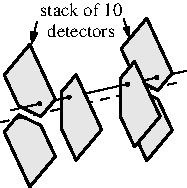
\includegraphics[height=0.3\textwidth]{../fig/stationScheme}}{(a)}\hfil
	\subtitle{\includegraphics[height=0.3\textwidth]{../fig/alignment_RP2}}{(b)}\hfil
	\subtitle{\includegraphics[height=0.3\textwidth]{../fig/es_profiles_bw}}{(c)}\hss
}%
\vskip-1mm
\caption{(a): An illustration of the detector overlap.
(b): A comparison of alignment results by the track based algorithm and the optical measurement.
(c): An example of a profile to determine the position of the beam -- a horizontal profile of elastic hits in a top RP, for $\be^* = 2\un{m}$ optics (the lowest elastic rate).
%(low acceptance for elastic events, hence low statistics).	
}%
\label{fig:align}%
\end{figure}




\begin{footnotesize}
\begin{thebibliography}{99}

\bibitem{tdr}
	TOTEM: Technical Design Report, CERN-LHCC-2004-002 (2004); addendum CERN-LHCC-2004-020.

\bibitem{jinst}
  G.~Anelli {\it et al.}  [TOTEM Collaboration],
  %``The Totem Experiment At The Cern Large Hadron Collider,''
  JINST {\bf 3}, S08007 (2008).

\bibitem{simone}
	S.~Giani [TOTEM Collaboration],
	{\it Diffraction at TOTEM},
	13$^{\rm th}$ International Conference on Elastic and Diffractive Scattering,
	CERN (2009).

\bibitem{tevatron1}
  F.~Abe {\it et al.}  [CDF Collaboration],
  %``Measurement of the $\bar{p}p$ total cross-section at $\sqrt{s} = 546$ GeV
  %and 1800-GeV,''
  Phys.\ Rev.\  {\bf D50} (1994) 5550.

\bibitem{tevatron2}
  N.~A.~Amos {\it et al.}  [E710 Collaboration],
  %``Measurement of $\rho$, the ratio of the real to imaginary part of the
  %$\bar{p} p$ forward elastic scattering amplitude, at $\sqrt{s}$ = 1.8-TeV,''
  Phys.\ Rev.\ Lett.\  {\bf 68} (1992) 2433.

\bibitem{gennaro}
	G.~Ruggiero [TOTEM Collaboration],
	{\it TOTEM},
	13$^{\rm th}$ International Conference on Elastic and Diffractive Scattering,
	CERN (2009).

\bibitem{cudell}
  J.~R.~Cudell {\it et al.}  [COMPETE Collaboration],
  %``Benchmarks for the forward observables at RHIC, the Tevatron-run II and
  %the LHC,''
  Phys.\ Rev.\ Lett.\  {\bf 89} (2002) 201801.
  %[arXiv:hep-ph/0206172].

\bibitem{mario}
	M.~Deile  [TOTEM Collaboration],
	{\it Total cross-section measurement and diffractive physics with TOTEM},
	12$^{\rm th}$ International Conference on Elastic and Diffractive Scattering,
	%Blois07, Forward physics and QCD* 153-159
	Hamburg (2007)

\bibitem{wy}
  G.~B.~West and D.~R.~Yennie,
  %``Coulomb interference in high-energy scattering,''
  Phys.\ Rev.\  {\bf 172} (1968) 1413.

\bibitem{kl}
  V.~Kundr\' at and M.~Lokaj\' i\v cek,
  %``High-energy scattering amplitude of unpolarized and charged hadrons,''
  Z.\ Phys.\ {\bf C63} (1994) 619.
  %%CITATION = ZEPYA,C63,619;%%

\bibitem{wy inconsistent}
  V.~Kundr\' at, M.~Lokaj\' i\v cek and I.~Vrko\v c,
  %``Limited validity of West and Yennie integral formula for elastic scattering
  %of hadrons,''
  Phys.\ Lett.\ {\bf B656} (2007) 182.
  %[arXiv:0706.0827 [hep-ph]].
  %%CITATION = PHLTA,B656,182;%%

\bibitem{millepede}
	V.~Blobel, Millepede II documentation at http://www.desy.de/$\sim$blobel/Mptwo.pdf\ .

\iffalse
\bibitem{alfa}
	ATLAS-ALFA: Technical Design Report, CERN-LHCC-2008-004 (2008).

\bibitem{ua5}
  G.~J.~Alner {\it et al.}  [UA5 Collaboration],
  %``Antiproton-proton cross sections at 200 and 900 {GeV} c.m. energy,''
  Z.\ Phys.\  {\bf C32} (1986) 153.
  %%CITATION = ZEPYA,C32,153;%%

\bibitem{isr}
  U.~Amaldi {\it et al.},
  %``The Energy dependence of the proton proton total cross-section for
  %center-of-mass energies between 23 and 53 GeV,''
  Phys.\ Lett.\  {\bf B44} (1973) 112.
\fi




\iffalse
\hrule
\bibitem{parton_qed} A.D.~Martin {\it et~al.}, Eur. Phys. J. {\bf C39} 155 (2005).
\bibitem{H1}N.~Gogitidze, arXiv:hep-ex/0701033 (2007).
\bibitem{DVCS}S.~Friot, B.~Pire and L.~Szymanowski, Phys. Lett. {\bf B645} 153 (2007);\\
              D.~Hasell, R.~Milner and K.~Takase, AIP Conf. Proc. {\bf 588} 187 (2001);\\
              M.~Krawczyk and A.~Zembrzuski, Phys. Rev. {\bf D57} 10 (1998).
\bibitem{pomeron}R.~Brower and C.~Tan, PoS LAT2005 279 (2006);\\
                 J.P.~Guillaud and A.~Sobol,
  {\it Perspectives of the study of double Pomeron exchange at the LHC},
  11th Lomonosov Conference on Elementary Particle Physics, Moscow, Russia (2003).
\fi

\end{thebibliography}

\end{footnotesize}


\end{document}
